

\actTitle{Worksheet 4.5A}

\noindent \textbf{Instructions:}  Work together in groups of  3 or 4 to complete the following problems.\\

Student goals:
\begin{itemize}
\item Determine the range and domain of a sine or a cosine function.
\item Determine the amplitude, period, and phase of a trigonometric
  function given a written or graphical representation.
\item Determine the vertical shift and scale of a trigonometric
  function given a written or graphical representation.
\item Graph a sine or cosine wave given a formula or written
  description.
\item Determine the formula for a sine or cosine wave given the
  graph or a written description of the function.
\end{itemize}

\begin{enumerate}

\item Determine the amplitude and period of the function.
\begin{enumerate}
\item $y=7\sin(2x)$ \vfill
\item $\displaystyle y=\frac{1}{7}\sin(2\pi x)$ \vfill
\item $\displaystyle y=-7\cos\left(-\frac{2}{3}x\right)$ \vfill
\end{enumerate}

\item Identify the phase shift and indicate whether the shift is to the left or to the right.
\begin{enumerate}
\item $\displaystyle \cos\left(x-\frac{\pi}{3}\right)$\vfill
\item $\displaystyle \cos\left(2x+\frac{\pi}{3}\right)$\vfill
\item $\displaystyle \sin\left(2\pi x -\frac{\pi}{8}\right)$\vfill
\end{enumerate}


\clearpage

\item Let $f(x)=2\cos(x+\pi)-1$.

\begin{enumerate}

\item Determine the period, amplitude, and phase shift of $f(x)=2\cos(x+\pi)-1$.\vfill
\item Find an interval containing exactly one cycle (period).\vfill
\item Determine the $x$-values of the five key points in the cycle above.
$$x_1= \quad \quad \quad \quad x_2= \quad \quad \quad \quad x_3= \quad \quad \quad \quad x_4= \quad \quad \quad \quad x_5= \quad \quad \quad \quad$$
\vfill





\item Graph $f(x)=2\cos(x+\pi)-1$.

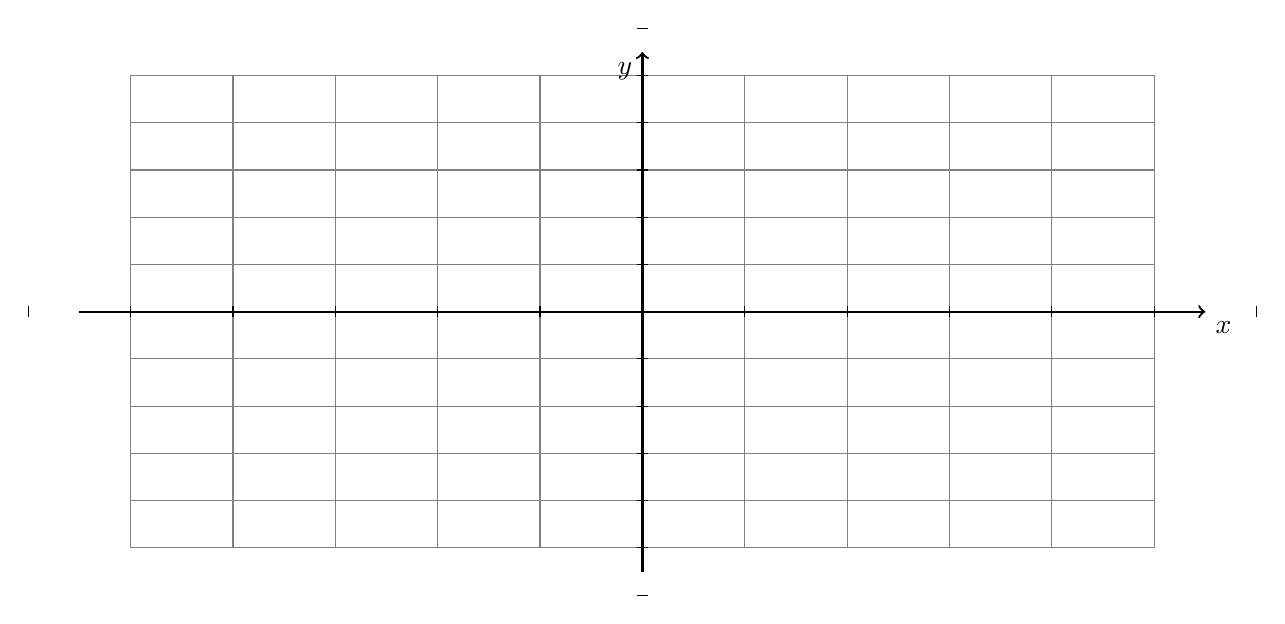
\begin{tikzpicture}[y=.6cm, x=1.3cm,font=\sffamily]
    %% ticks
    \draw[step = 1, gray] (-5,-5) grid (5,5);
    %% axis
    \draw[thick,->] (-5.5,0) -- coordinate (x axis mid) (5.5,0) node[anchor = north west] {$x$};
    \draw[thick,->] (0,-5.5) -- coordinate (y axis mid) (0,5.5) node[anchor = north east] {$y$};
    \foreach \y in {-6,-5,...,-1,1,2,...,6} {
      \draw (2pt, \y) -- (-2pt, \y);
    }
    \foreach \x in {-6,-5,...,-1,1,2,...,6} {
      \draw (\x,2pt) -- (\x,-2pt);
    }

  \end{tikzpicture}

\end{enumerate}


\clearpage

\item The function $y=a\sin(x)+d$ has range $[-10,28]$.  Assuming that $a$ is positive, determine the values for $a$ and $d$.

\vfill
\item The function $y=a\cos(x)+d$ has range $[-26,10]$.  Assuming that $a$ is positive, determine the values for $a$ and $d$.
\vfill

\item Let $f(x)=-7\sin(6x)$.
\begin{enumerate}
\item Determine the coordinates $(x,y)$ of the first maximum turning point on the graph $f(x)$ in the interval $(0,2\pi)$.
\vfill

\item Determine the coordinates $(x,y)$ of the first minimum turning point on the graph $f(x)$ in the interval $(0,2\pi)$.
\vfill

\end{enumerate}

\clearpage

\item The displacement of one of the vibrating wires in a piano is
  \begin{eqnarray*}
    D(t) & = & 0.05\cos\left(0.1\frac{\sqrt{T}}{L} t \right),
  \end{eqnarray*}
  where $T$ is the tension in the wire (measured in Newtons), $L$ is
  the length of the wire (meters), and $t$ is the time. A piano maker
  wishes to make a wire that vibrates 500 cycles per second, and the
  length of the wire will be 0.9 meters. What tension will be
  required?



\end{enumerate}


\hwTitle{Section 4.5A}

\begin{enumerate}
\item Let $\displaystyle f(x)=-5\sin\left(\frac{1}{3}x+\frac{\pi}{6}\right)$.

\begin{enumerate}

\item Determine the period, amplitude, and phase shift of
  $\displaystyle f(x)=-5\sin\left(\frac{1}{3}x+\frac{\pi}{6}\right)$.
\item Find an interval containing exactly one cycle (period).
\item Determine the $x$-values of the five key points in the cycle above.
$$x_1= \quad \quad \quad \quad x_2= \quad \quad \quad \quad x_3= \quad \quad \quad \quad x_4= \quad \quad \quad \quad x_5= \quad \quad \quad \quad$$
\item Graph $\displaystyle f(x)=-5\sin\left(\frac{1}{3}x+\frac{\pi}{6}\right)$.

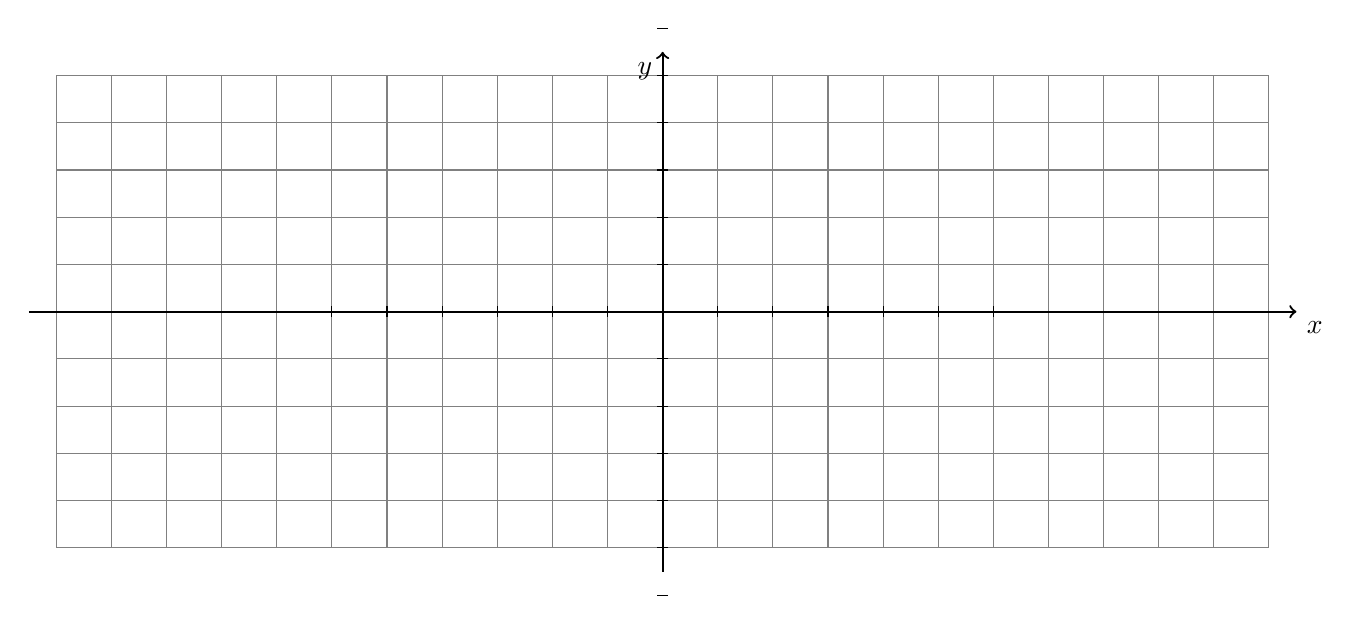
\begin{tikzpicture}[y=.6cm, x=.7cm,font=\sffamily]
    %% ticks
    \draw[step = 1, gray] (-11,-5) grid (11,5);
    %% axis
    \draw[thick,->] (-11.5,0) -- coordinate (x axis mid) (11.5,0) node[anchor = north west] {$x$};
    \draw[thick,->] (0,-5.5) -- coordinate (y axis mid) (0,5.5) node[anchor = north east] {$y$};
    \foreach \y in {-6,-5,...,-1,1,2,...,6} {
      \draw (2pt, \y) -- (-2pt, \y);
    }
    \foreach \x in {-6,-5,...,-1,1,2,...,6} {
      \draw (\x,2pt) -- (\x,-2pt);
    }

  \end{tikzpicture}

\end{enumerate}


\end{enumerate}
